\section{Attributing temporary network admission to a single request}
\label{sec:method}

For a target request, resource, and observation window, the method reports how the system processed the request and what effect the request had. Attribution proceeds in two stages. We first ask whether the target triggered a successful operation. We then ask whether that operation established new admission to the resource. The first judgment must accommodate ambiguity about which request initiated each operation. The second must rule out access under an existing rule or one installed by another request. The control and data paths define the observation boundary. Within that boundary, the two tests use different evidence.

\subsection{Execution path and observation model}
\label{sec:observation}

OpenNHP implements the Network-Infrastructure Hiding Protocol (NHP). Its control plane verifies knocks, processes authorization decisions and configures temporary access. Its data plane applies the active rules to application traffic. An Authorization Service Provider (ASP) may make the policy decision, and the Access Controller (NHP-AC) enforces it. The path evaluated here uses the example authorization plugin in the NHP-Server process. We follow the NHP message terminology~\citep{r39}.

The Agent sends a knock (KNK, step~1). NHP-Server verifies the message and invokes the plugin. When the resource should be opened, the Server sends an open request (AOP) to the AC (step~2). The AC writes a short-lived rule (step~3) and returns the result (ART). The Server returns a knock acknowledgment (ACK) to the Agent. This exchange determines whether a rule operation is requested and completed. The application client then opens a separate TCP connection (step~4). The kernel checks the source address, target resource and rule validity period. It forwards matching traffic to the protected service (step~5) and drops unmatched traffic by default in this deployment. The HTTP response returns over the application connection. The temporary rule links the two paths, as shown in Fig.~\ref{fig:1}.

\begin{figure*}[t]
\centering
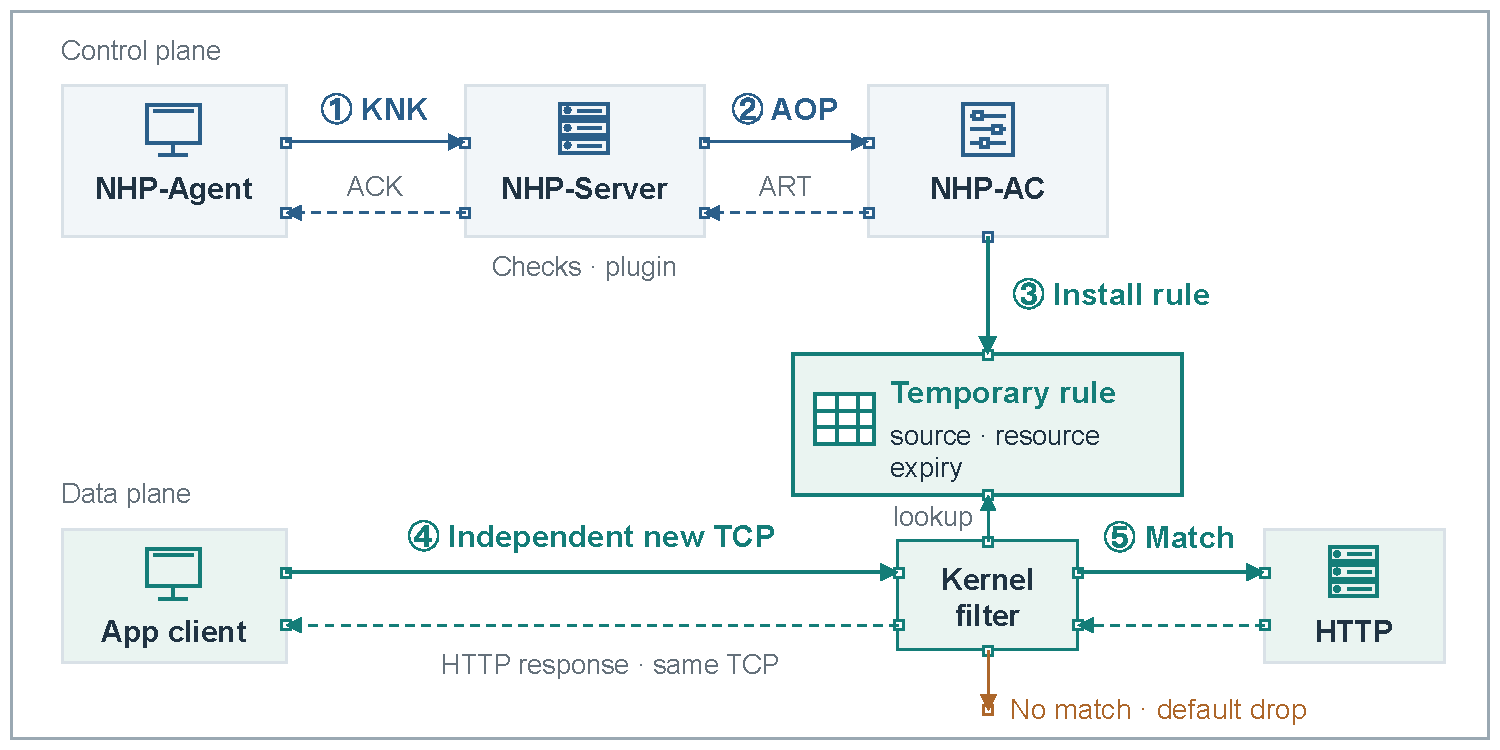
\includegraphics[width=\textwidth]{fig1.pdf}
\caption{Temporary admission in OpenNHP. (1) The Agent sends a knock. (2) The Server asks the AC to open access. (3) The AC installs a short-lived rule. (4) The application client opens a new TCP connection. (5) The kernel forwards matching traffic to the protected service.}
\label{fig:1}
\end{figure*}

These paths determine what must be observed. Control-plane records identify requests and the operations they may have initiated. Rule records establish the state of the resource. Independent probes check service health and the outcome of a fresh connection. An application response does not identify the request that installed the rule, and a control response cannot establish whether a new application connection succeeded. To attribute admission, we link observations of the request, rule, and connection in event order. Section~\ref{sec:setup} describes the collection interfaces.

The unit of attribution is one receipt of a KNK message for a given resource within a given window. The same bytes can be received more than once. We distinguish requests by the receive instance and its connection scope, and compare packet contents by fingerprint. Two receipts remain separate even when their transaction identifiers or contents coincide. Conversely, a single callback can issue several related rule commands. We treat those commands as one \emph{action bundle}, the unit to which both source attribution and capacity constraints apply.

The observation model allows repeated delivery of captured messages, changes of connection, unconfigured keys and modified ciphertext. It also allows configured participants to request the same resource at nearly the same time. We trust the collector records, process-start identities, verified transaction links, operation outcomes and resource probes. The adversary cannot alter these records or forge a trusted link. Instrumentation records links along the execution path within each process, from a receive instance to an action bundle. A verified relation serves as an explicit request link.

The observation boundary covers requests and actions relevant to the same resource, path and window. It also accounts for asynchronous writes and rules that took effect before the window and remain active. Request coverage, action coverage and any bound on the number of bundles attributable to a request must be justified over that boundary. Where a condition cannot be verified, the model retains the alternatives it would otherwise exclude.

\subsection{Candidate associations and target-action judgments}
\label{sec:target-action}

We use the observations to construct a bipartite graph of candidate associations. Feasibility queries then determine whether the target's success is necessary or possible without enumerating all compatible explanations. Figure~\ref{fig:2} illustrates this with complete request records. Two requests, $q$ and $u$, are the only possible sources of two known successful bundles. Each request can account for at most one bundle. Both assignments are feasible, and each gives $q$ a successful action. The target's outcome is therefore determinate even though either bundle could belong to it.

\paragraph{1. Construct the candidate graph.}
For a target request $q$, resource $r$ and observation window $W$, receive, rejection and application-processing events provide the request set $Q$. Execution records provide the set $A$ of action bundles. Each bundle $a$ has a resource, a candidate source domain $D(a)$ and an outcome $s_a\in\{1,0,?\}$ denoting success, no success or an unknown result. For example, the related rule commands arising from one AOP form one bundle. For native KNK, a successful bundle requires a completed AC write, successful execution of every expected rule command, a successful ART, and a consistent terminal status at the Server. We record an action bundle as unsuccessful only if the write explicitly failed and no rule was added successfully. An incomplete outcome chain remains unknown. If only part of a bundle succeeds, the run is separately flagged as a collection anomaly and handled by the inclusion criteria.

The graph places bundles on one side and requests on the other. An edge requires agreement on the resource and compatibility with the connection, transaction and bounded processing interval. The edge identifies a possible source. A verified unique link along the execution chain fixes the source. If only the processing interval identifies a single candidate, source attribution also requires request coverage. A request is excluded as a source only when a recorded rejection occurred at a receive checkpoint capable of preventing the modeled operation. A backend error after application processing began is assessed from the processing and action records. If a verified explicit link uniquely identifies a request that was rejected at the relevant checkpoint, the evidence conflicts. Edges restrict possible sources, and outcome labels restrict possible effects. Step~1 of Fig.~\ref{fig:2} encodes both constraints. Step~2 asks whether all bundles can be assigned under those constraints.

\begin{figure*}[t]
\centering
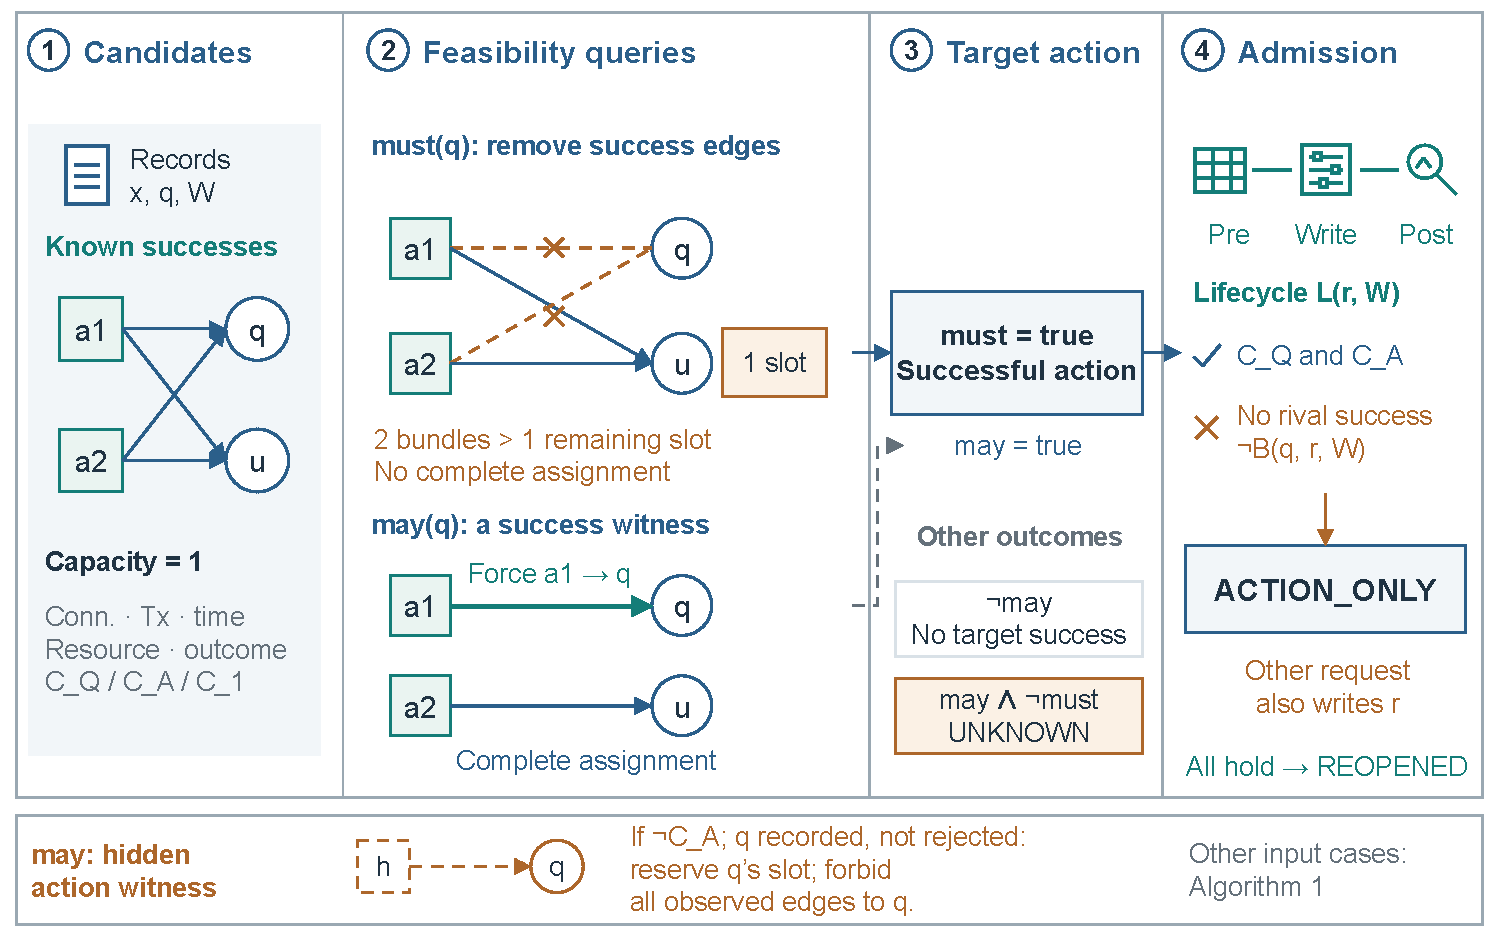
\includegraphics[width=\textwidth]{fig2.pdf}
\caption{Two-stage attribution for a recorded target with known processing status. Candidate associations (1) and feasibility queries (2) determine target success (3). A competing write to the same resource limits the example to \texttt{ACTION\_ONLY} at the admission check (4). The bottom row shows how an unrecorded action can witness possible success.}
\label{fig:2}
\end{figure*}

Three observation conditions govern what can be inferred from missing records. \emph{Request coverage}, $C_Q$, means that all requests that could initiate an action within scope have been recorded. Without verified request coverage, each bundle lacking a unique explicit link retains its own unobserved source. The model does not require different bundles to share that source. \emph{Action coverage}, $C_A$, means that all relevant bundles within scope have been recorded. If action coverage is unconfirmed, a recorded target that was not explicitly rejected may have one unrecorded successful action.

The \emph{unit-capacity condition}, $C_1$, permits at most one bundle per request. Observed and admissible hidden actions share this capacity. Assigning one bundle can therefore constrain the assignment of another. Source code and configuration must support the bound, and the run records are checked for violations. Where the bound lacks support, we impose no upper limit. Neither the coverage conditions nor the capacity bound follows from the absence of additional log entries.

If $q\notin Q$, the base graph must first admit a feasible assignment. Given feasibility and $C_Q$, the processing status is \texttt{NO\_TARGET\_RECORD} and the effect is \texttt{NO\_TARGET\_ACTION}. If $C_Q$ is unconfirmed, the target might have occurred without being recorded, so both fields are \texttt{UNKNOWN}. In either case, the reported values of $\operatorname{must}$ and $\operatorname{may}$ are inapplicable. This branch neither identifies a bundle's private external source as the target nor adds a hidden successful action for an unidentified target.

These constraints define the candidate graph $G=(A,Q\cup U,E,s,c)$. The set $U$ contains unobserved sources. If request coverage is unconfirmed, each bundle $a$ without a unique explicit source retains a private node $u_a$. After explicitly rejected sources have been excluded, $D(a)$ denotes the remaining candidate domain, and $E=\{(a,v):v\in D(a)\}$. For a request $v$, $c(v)=1$ under $C_1$ and is otherwise unbounded. Each external node has $c(u_a)=1$ and is adjacent only to its own bundle. It introduces no competition for capacity between bundles. If a verified unique source was explicitly rejected, its bundle has an empty domain, which yields a conflict.

A compatible explanation is a tuple $\omega=(f,z,h)$: $f$ assigns sources to observed bundles, $z$ completes their unknown outcomes, and $h\in\{0,1\}$ indicates whether a successful target action is missing from the record. The space $\Omega$ comprises the tuples satisfying the following constraints:
\begin{itemize}
\item \emph{Source.} For every $a\in A$, $f(a)\in D(a)$.
\item \emph{Outcome.} $z_a\in Z_a$, where $Z_a=\{s_a\}$ for a known outcome and $Z_a=\{0,1\}$ otherwise.
\item \emph{Unrecorded action.} The value $h=1$ is permitted only if action coverage is unconfirmed and the target is recorded and was not explicitly rejected. Otherwise $h=0$.
\item \emph{Capacity.} For every $v\in Q\cup U$,
\[
   \sum_{a\in A}\mathbf{1}[f(a)=v]+h\mathbf{1}[v=q]\le c(v).
\]
\end{itemize}

The target query asks whether at least one action succeeded. A single unrecorded success suffices as a witness and consumes the corresponding capacity at the target. Define $S(q,\omega)\iff h=1\lor\exists a\in A:\ f(a)=q\land z_a=1$. To report the action predicates, the target must be known to have entered application processing or to have been explicitly rejected. In native KNK, entry into the plugin callback confirms application processing; receipt of a packet alone leaves that status open. For $\Omega\ne\varnothing$, $q\in Q$ and determinate processing status, define
\begin{equation}
  \operatorname{must}(q)\iff\forall\omega\in\Omega,\ S(q,\omega).
  \label{eq:must}
\end{equation}
\begin{equation}
  \operatorname{may}(q)\iff\exists\omega\in\Omega,\ S(q,\omega).
  \label{eq:may}
\end{equation}
Equation~\eqref{eq:must} requires target success in every explanation. Equation~\eqref{eq:may} requires target success in at least one explanation. The successful bundle can differ between explanations. This use of certain-answer semantics retains ambiguity about the underlying associations~\citep{r38}. If the base graph admits no assignment, the method reports a conflict before evaluating necessity over an empty explanation space.

\paragraph{2. Test necessary and possible success.}
With unit capacity, feasibility reduces to a bipartite matching that covers every action bundle~\citep{r40}. The implementation uses depth-first search (DFS) to find an augmenting path for each bundle. Under unbounded request capacity, it suffices to check that each bundle has at least one candidate. Once the base graph is feasible, we use the two queries in Fig.~\ref{fig:2}.

The edge-deletion query asks whether the target can have no successful action. Delete every edge to $q$ from a bundle known to have succeeded. If the remaining graph still admits an assignment, assign a nonsuccessful outcome to the target's unknown bundles and omit the optional hidden success. The resulting explanation shows that the target can have no successful action. If the reduced graph is infeasible, every compatible explanation assigns at least one known successful bundle to $q$, establishing $\operatorname{must}(q)$.

The forced-edge query asks whether the target can have a successful action. Force, in turn, each edge to $q$ whose bundle permits success and test whether the other bundles still admit an assignment. If the model permits a hidden success at $q$, also test feasibility with that action present. Under unit capacity the hidden action occupies the target's only slot, so all observed bundles must be assigned elsewhere. Any such feasible assignment establishes $\operatorname{may}(q)$.

\paragraph{3. Determine the target-action outcome.}
Necessary success triggers the resource check. If explanations with and without success are both feasible, the effect remains unknown. If no successful explanation exists, the target has no successful action. The solver retains the corresponding witness, counterexplanation or observation gap. In Fig.~\ref{fig:2}, deleting all known-success edges to the target leaves both bundles competing for the other request's single slot, proving necessary success. Hall's condition provides a check on such a capacity deficit: if a subset $S$ of bundles has a candidate neighborhood $N(S)$ with $|N(S)|<|S|$, no assignment can cover all bundles in $S$~\citep{r41}.

Singleton propagation fixes individual assignments. A global feasibility query can determine the target outcome even when individual assignments remain interchangeable. With complete request records, propagation can assign a bundle with only one candidate source, use that request's capacity, and thereby resolve other bundles, as in the upper row of Fig.~\ref{fig:3}. In the lower row, both known successful bundles have the same two candidate requests and there are no external sources. Their assignments can be exchanged, but unit capacity gives each request a success in every assignment. In the figure, M is our global query, B1 is local propagation, B2 is exact enumeration and B3 is a minimum-cost flow method. Section~\ref{sec:setup} describes the comparison.

\begin{figure*}[t]
\centering
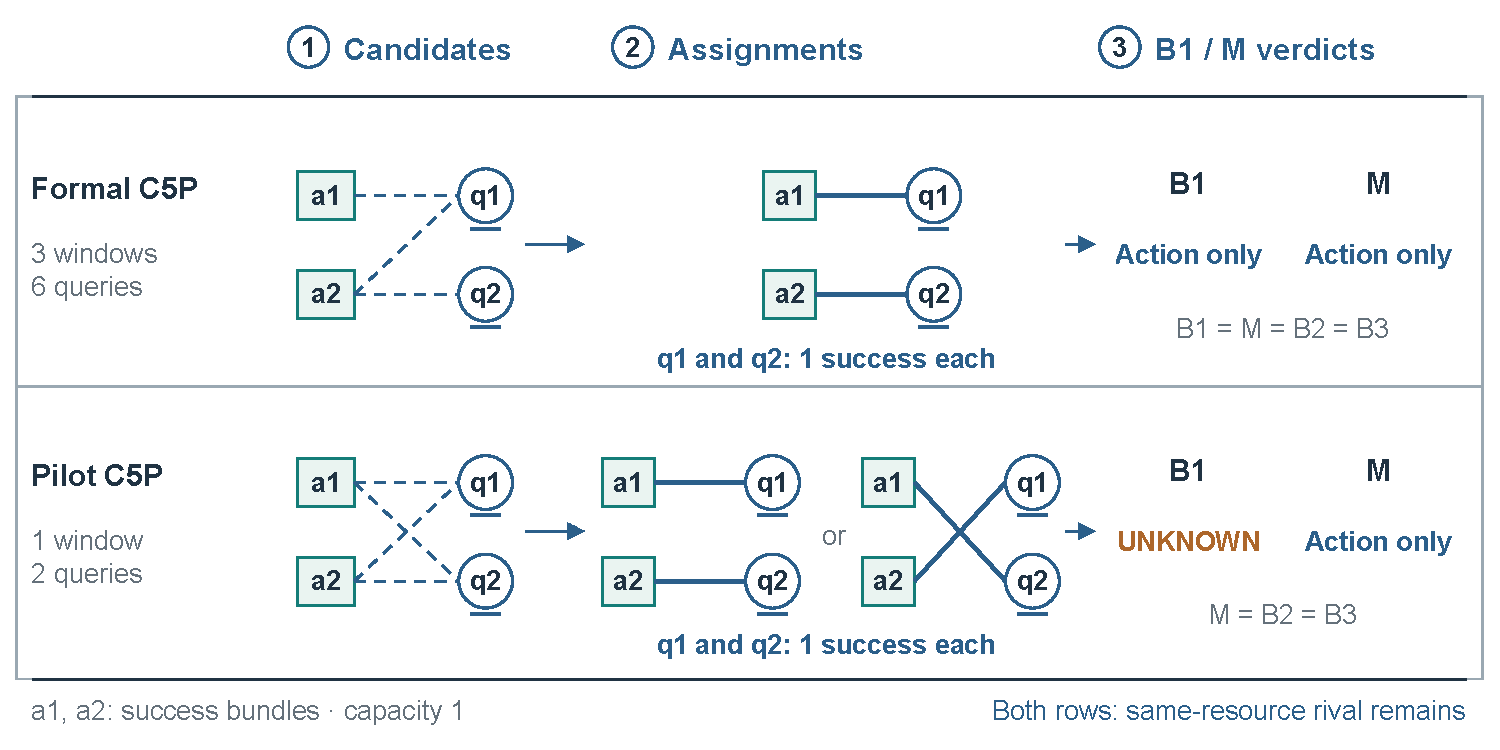
\includegraphics[width=\textwidth]{fig3.pdf}
\caption{Candidate structure and target outcome. Both the formal synchronized C5P windows (Formal C5P) and the separate engineering pilot (Pilot C5P) contain competing writes. Columns (1)--(3) show candidate sources, feasible assignments, and the verdicts of local propagation (B1) and global queries (M). ``Action only'' denotes \texttt{ACTION\_ONLY}.}
\label{fig:3}
\end{figure*}

The upper row supplies a singleton from which propagation can begin. In the lower row, propagation stops, but graph-wide capacity still constrains the target outcome. Edge deletion tests whether the remaining source domains and capacities can all be satisfied at once. Any additional determinate verdict therefore depends on the outcome labels, the target and the observation conditions as well as the candidate graph. In both rows, a successful write by another request remains a competing explanation for admission. The second stage examines the resource transition and its possible sources.

\subsection{Verifying new admission}
\label{sec:new-admission}

A successful write establishes new admission only under additional conditions. A rule already active before the write could explain a later successful connection. Even if the resource was closed beforehand, another request could have opened it. Ruling out these alternatives requires evidence of a resource-state transition and a check for competing writes.

\paragraph{4. Check the resource transition and competing explanations.}
Before the write, the rule set must be empty, a fresh external TCP probe must fail, and the service must be healthy. All three observations must precede the write. Together they establish the closed state and distinguish it from service failure. After the write, the probe must use a fresh connection, the HTTP response must meet the success criterion, and the probe must follow the write. Let $\ell_1,\ldots,\ell_7$ represent the pre-write predicates \texttt{rule\_empty}, \texttt{tcp\_failed}, \texttt{health\_ok} and \texttt{order\_ok}, followed by the post-write predicates \texttt{new\_tcp}, \texttt{http\_ok} and \texttt{order\_ok}. Then $L(r,W)=\bigwedge_{i=1}^{7}\ell_i$, with every predicate required to be explicitly true. The native adapter verifies the predicates using command times, phase order, rule readback and connection evidence. The solver takes the verified Boolean values as input. Appendix~A defines the fields.

Once the lifecycle conditions hold, the method checks whether some compatible explanation admits a successful write by a nontarget request to the same resource. Denote this condition by $B(q,r,W)$. The exclusion rule is conservative at the granularity of the input's resource identifier: as long as a competing success on the same resource within the window remains possible, admission cannot be attributed to the target alone. For a recorded target with determinate processing status, new admission requires
\begin{equation}
\begin{aligned}
\operatorname{admit}(q,r,W)={}&\operatorname{must}(q)\land L(r,W)\\
 &{}\land C_Q\land C_A\land\neg B(q,r,W).
\end{aligned}
\label{eq:admit}
\end{equation}
Here $\operatorname{must}(q)$ establishes target success and $L(r,W)$ establishes the resource transition. The two coverage conditions exclude missing sources and actions within scope. The final predicate excludes competing sources within the model. This last test reuses forced-edge queries: it forces each potentially successful nontarget edge for the same resource in turn. Any feasible assignment retains a competing explanation and limits the verdict to \texttt{ACTION\_ONLY}.

In native KNK runs, the rule is read back independently between the write and the application probe to check its source address, destination address and TCP port. An HTTP~200 response on a new connection then confirms successful application access. These checks are retained when building the method input. Both first admission and admission re-established after expiry receive the label \texttt{REOPENED}. The observation boundary includes asynchronous writes and rules that remain active from before the window.

Table~\ref{tab:2} lists the possible effects. If target success is necessary but a condition for new admission is missing or unverified, the method reports action success alone. Processing status is recorded separately so that rejection at the receiver can be distinguished from application processing without successful execution. Authorization conformance is a subsequent mapping $\operatorname{Auth}_{\rho}(e)$ from effect $e$ under a rule $\rho$. It has no role in source or admission attribution. Mapping requires an applicable native rule or test-reference policy, a nonempty provenance field and a Boolean permission flag. With no successful target action, the protected effect shows no deviation in that instance. For action success or established admission, the outcome conforms or deviates according to whether the rule permits the target. An invalid rule or unresolved effect leaves conformance unresolved. The implementation records native and test-reference provenance separately. Independent controls check that legitimate requests retain their functionality. If a rule separately requires explicit rejection at the receiver, we also check that requirement against the processing status.

\begin{table*}[t]
\centering
\caption{Execution effects for a designated request.}
\label{tab:2}
\begin{tabularx}{\textwidth}{@{}p{0.27\textwidth}X@{}}
\toprule
Execution effect & Condition \\
\midrule
Admission established\newline\texttt{REOPENED} &
Target success is necessary, the lifecycle observations and both coverage conditions hold, and competing successful writes to the same resource are excluded.\\
Action success only\newline\texttt{ACTION\_ONLY} &
Target success is necessary, but at least one condition for attributing new admission has not been established.\\
No successful target action\newline\texttt{NO\_TARGET\_ACTION} &
Processing status is known and no compatible explanation gives the target a success. This effect also applies when request records are complete and contain no target; processing status then records the absence of the target, and both action predicates are inapplicable.\\
Unresolved\newline\texttt{UNKNOWN} &
Target processing is unobserved, or explanations with and without target success are both compatible.\\
Conflict\newline\texttt{CONFLICT} &
No feasible assignment covers the observed bundles.\\
\bottomrule
\end{tabularx}
\end{table*}

Algorithm~\ref{alg:attribution} connects target-action queries with admission verification. For an assignment $f$ that covers all observed bundles and satisfies the candidate and capacity constraints, write $E_f=\{(a,f(a)):a\in A\}$. For forced and forbidden edge sets $P,N\subseteq E$, the feasibility query $F(P,N)$ is true if and only if such an assignment exists with $P\subseteq E_f$ and $E_f\cap N=\varnothing$. Omitted arguments default to the empty set. The implementation forces at most one candidate edge at a time, so a forced edge in the pseudocode denotes its singleton set. The query assigns only observed bundles. The separate hidden-success test accounts for a possible unrecorded success.

\newcounter{nhpalgorithm}
\begin{figure*}[t]
\refstepcounter{nhpalgorithm}\label{alg:attribution}
\centering
\begin{minipage}{\textwidth}
\small
\textbf{Algorithm \thenhpalgorithm. Single-request action classification and new-admission verification}\par\smallskip
\begin{tabularx}{\linewidth}{@{}r@{\quad}X@{}}
\toprule
\multicolumn{2}{@{}p{0.98\linewidth}@{}}{\textbf{Input:} normalized observations $x$, target $q$ and conditions $C_Q,C_A,C_1$.}\\
\multicolumn{2}{@{}p{0.98\linewidth}@{}}{\textbf{Output:} run status, processing status $p$, effect, authorization conformance, applicable values of $\operatorname{must}$ and $\operatorname{may}$, and an audit record.}\\
\midrule
& \textit{Validate the input and base graph}\\
01 & Validate $x$; on failure, return \texttt{INVALID\_INPUT}.\\
02 & Set $p$ to the recorded target's processing status. If absent, use \texttt{NO\_TARGET\_RECORD} when $C_Q$ holds and \texttt{UNKNOWN} otherwise.\\
03 & Construct $G$. Use $F(\mathrm{force},\mathrm{forbid})$ to test feasibility and retain a witness.\\
04 & If $\neg F()$, return \texttt{CONFLICT}.\\
& \textit{Stage 1: determine target-action success}\\
05 & $\mathrm{must}\gets\neg F(\mathrm{forbid}=\{\text{all known-success edges to }q\})$.\\
06 & $\mathrm{may}\gets\mathrm{false}$.\\
07 & For each edge $(a,q)$ whose outcome permits success:\\
08 & \hspace*{1em}If $F(\mathrm{force}=(a,q))$, set $\mathrm{may}\gets\mathrm{true}$ and break.\\
09 & If $C_A$ is unconfirmed, $q$ is recorded and $p\ne\texttt{REJECTED}$:\\
10 & \hspace*{1em}$\mathrm{hidden}\gets (\text{request capacity is unbounded})\lor F(\mathrm{forbid}=\{\text{all edges to }q\})$.\\
11 & \hspace*{1em}$\mathrm{may}\gets\mathrm{may}\lor\mathrm{hidden}$.\\
& \textit{Stage 2: verify new admission}\\
12 & Set $L$ to the conjunction of the seven lifecycle predicates and $B\gets\mathrm{false}$.\\
13 & If $\mathrm{must}\land L\land C_Q\land C_A$:\\
14 & \hspace*{1em}For each potentially successful nontarget edge $(a,v)$ for the same resource:\\
15 & \hspace*{2em}If $F(\mathrm{force}=(a,v))$, set $B\gets\mathrm{true}$ and break.\\
& \textit{Classify the effect and map authorization}\\
16 & If $p=\texttt{UNKNOWN}$, set $\mathrm{effect}\gets\texttt{UNKNOWN}$.\\
17 & Else if $p=\texttt{NO\_TARGET\_RECORD}$, set $\mathrm{effect}\gets\texttt{NO\_TARGET\_ACTION}$.\\
18 & Else if $\mathrm{must}$, set $\mathrm{effect}$ to \texttt{REOPENED} when $L\land C_Q\land C_A\land\neg B$ holds and to \texttt{ACTION\_ONLY} otherwise.\\
19 & Else if $\neg\mathrm{may}$, set $\mathrm{effect}\gets\texttt{NO\_TARGET\_ACTION}$.\\
20 & Else set $\mathrm{effect}\gets\texttt{UNKNOWN}$.\\
21 & Save witnesses, counterexplanations and unmet observation conditions.\\
22 & Map the effect to authorization conformance under the applicable rule.\\
23 & If $q$ is unrecorded or $p=\texttt{UNKNOWN}$, report $\mathrm{must}$ and $\mathrm{may}$ as inapplicable.\\
24 & Return run status, $p$, effect, authorization conformance, applicable $\mathrm{must}/\mathrm{may}$ and the audit record.\\
\bottomrule
\end{tabularx}
\end{minipage}
\end{figure*}

Line~5 forbids only known-success edges to the target. The target may still receive a failed bundle, or one whose unknown outcome can be set to failure. This tests for a counterexample to necessary success. Line~10 forbids \emph{all} edges to the target under unit capacity. It reserves the only slot for a hidden success, so even a known failure or an unknown bundle must be assigned elsewhere.

\subsection{Conditional correctness and computational complexity}
\label{sec:correctness}

The two action queries must agree with the definitions in Eqs.~\eqref{eq:must} and~\eqref{eq:may}. Let $\omega^\ast$ denote the projection of the actual execution. If records are authentic, each candidate set contains the true source, verified explicit links are correct, and the asserted coverage and capacity conditions hold, then $\omega^\ast\in\Omega$. The following propositions assume that the base graph is feasible, the target is recorded and its processing status is determinate.

\paragraph{Proposition 1 (necessary success).}
The graph has no feasible assignment after removal of all known-success edges to the target if and only if every compatible explanation assigns a successful action to that target.

\emph{Proof.} If the reduced graph admits an assignment, give any unknown bundle assigned to the target a nonsuccessful outcome and omit the optional hidden success. This yields an explanation without target success. Conversely, any explanation without target success uses none of the deleted edges, and its assignment remains feasible after deletion. Infeasibility thus excludes exactly the counterexamples. Since $\omega^\ast\in\Omega$, necessary success also holds for the actual execution.

\paragraph{Proposition 2 (possible success).}
A successful target explanation exists if and only if either a potentially successful target edge can be forced in a feasible assignment, or the model permits an unrecorded successful target action and the remaining assignment is feasible.

\emph{Proof.} Every explanation with target success contains at least one of the two witnesses. Conversely, a feasible forced-edge assignment permits success for its associated bundle. An admissible hidden action can likewise witness success. Under unit capacity, that hidden action consumes the target's slot. If every assignment already fills it with an observed bundle, incomplete action records alone cannot establish possible success through a hidden action.

The propositions establish necessity and possibility for action success under the stated model. Equation~\eqref{eq:admit} additionally tests the resource transition and competing writes for admission. A separate policy mapping then determines whether the observed effect conforms to the applicable authorization rule.

\paragraph{Computational complexity.}
Let $n=|A|$ and $e=|E|$, including admissible external sources. Algorithm~\ref{alg:attribution} makes at most $e+3$ feasibility checks. The base graph, the known-success deletion and the hidden-success test require at most one check each. Forced edges for target success and competing success belong to disjoint sets, so together they require at most $e$ further checks. With the current DFS augmenting-path implementation, one matching visits $O(ne)$ edges; all queries together visit $O((e+3)ne)$ edges. An empty bundle set is immediately feasible. Building candidate domains and checking for empty domains contribute separate linear work. The implementation also sorts bundles and candidates to obtain a stable traversal order. With maximum candidate domain size $\Delta$, a conservative per-check time bound is $O(n+e+n\log(2+n)+ne\log(2+\Delta))$. Storing the graph and the matching requires $O(|Q|+n+e)$ space. Section~\ref{sec:cost} reports measured query counts and invocation times.
